\section{Lenkung anhand der Linien} % Bitte sinnvolle Überschriften für alle Kapitel und Unterkapitel wählen
\subsection{Die erste „naive“ Idee und ihre Probleme}
Zur Erkennung und Auswertung der Linien arbeiten wir mit Canny Edge zur Kantenerkennung und Houghline, um daraus Linien zu erkennen.Zu Beginn des Projektes hatten wir über verschiedene Ansätze nachgedacht, wie wir den Lenkwinkel anhand der vorhandenen Verkehrslinien bestimmen können. Einer dieser frühen „naiven“ Ansätze war den Lenkwinkel anhand eines „durchschnittlichen Vektor“ zu bestimmen, der sich aus den rechts und links von Houghline erkannten Vektoren zusammen setzt. Der Lenkwinkel sollte dann der Winkel zwischen diesem Vektor und der X-Achse sein. 
\begin{figure}[H]
	\centering	
	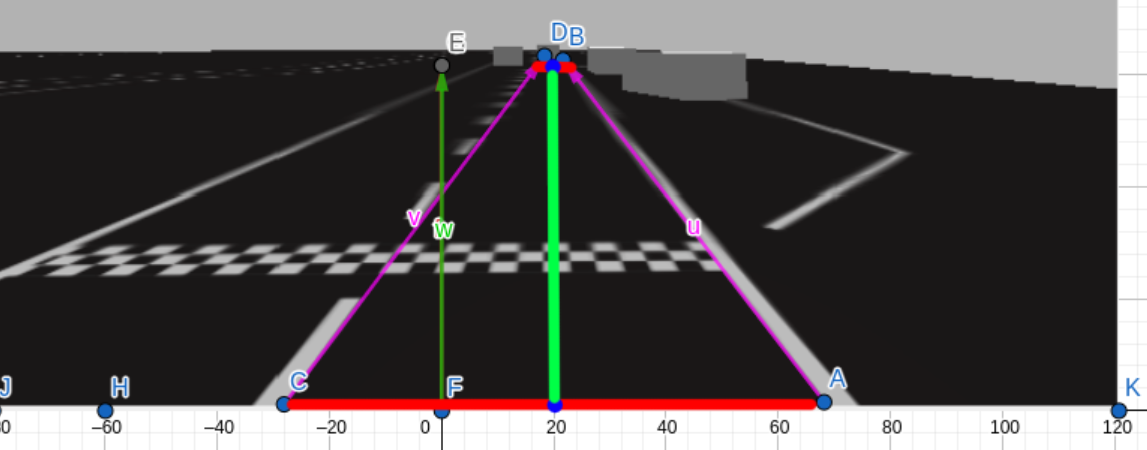
\includegraphics[width=.5\textwidth]{img/vector_gerade}
	\caption[durchschnittlichen Vektor am Start]{durchschnittlichen Vektor am Start}
	%\captionsource{So könnte man z.b. die Bildquelle angeben}
	\label{fig:vector_gerade}
\end{figure}

Diese „naive“ Idee wurde beim ersten Testen in GeoGebra bereits schnell wieder verworfen. Das Problem hierbei ist, dass wir eigentlich außerhalb von Kurven  den Vektor gespiegelt um die Y-Achse bräuchten, um zur Soll-Fahrbahn zu lenken. In den Kurven wiederum brächten wir wieder den zuvor genannten „Durchschnittsvektor“. Daher haben wir das ganze schnell wieder verworfen, aber konnten daraus eine andere Idee entwickeln.

\begin{figure}[H]
	\centering	
	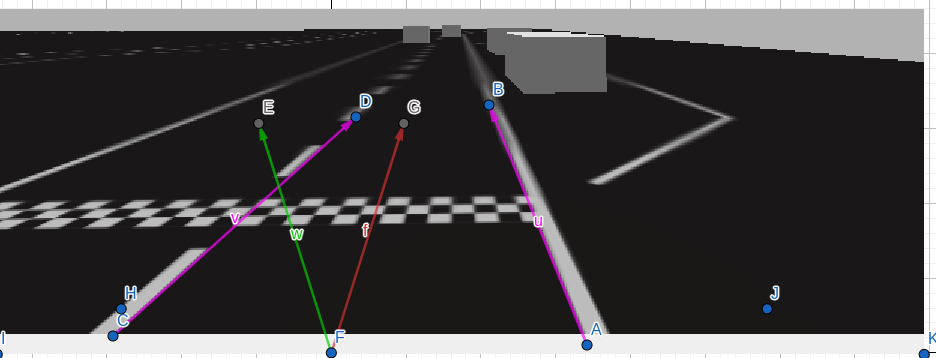
\includegraphics[width=.5\textwidth]{img/vector_zu_rechts}
	\caption[durchschnittlichen Vektor wenn zu weit rechts auf der Geraden]{durchschnittlichen Vektor wenn zu weit rechts auf der Geraden}
	%\captionsource{So könnte man z.b. die Bildquelle angeben}
	\label{fig:vector_zu_rechts}
\end{figure}

\begin{figure}[H]
	\centering	
	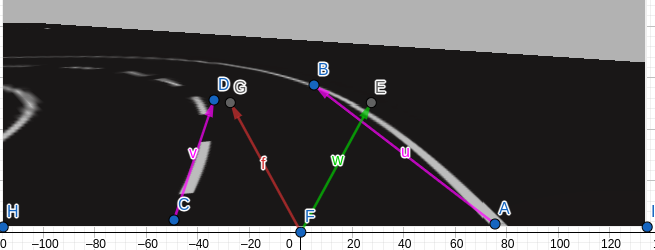
\includegraphics[width=.5\textwidth]{img/vector_kurve}
	\caption[durchschnittlichen Vektor in Kurve]{durchschnittlichen Vektor in Kurve}
	%\captionsource{So könnte man z.b. die Bildquelle angeben}
	\label{fig:vector_kurve}
\end{figure}

\begin{itemize}
			\item \color{red} Rot $\Rightarrow$ Durchschnittsvektor 	\qquad \color{green} Grün $\Rightarrow$ gespiegelter Durchschnittsvektor
			
\end{itemize}



\subsection{Weiterentwicklung der ersten Idee}
Nach Reflektieren unseres ersten Ansatzes stellten wir fest, dass uns die Y-Koordinate eigentlich egal sein kann und dass wir lediglich eine X-Koordinate benötigen, um zu wissen, ob wir nach links oder rechts lenken müssen. So kam uns die Idee, einfach den Durchschnitt aus den linken und rechten X-Koordinaten, die durch Houghline erkannt wurden, zu bilden und anhand dessen die Fahrbahn zu bestimmen. Die Idee hierbei war, die X-Koordinate der Bildmitte, die auch die Mitte des Autos ist, einfach mit der errechneten X-Koordinate zu vergleichen und anhand dessen zu lenken.

Das Ganze haben wir zunächst mit der Mittellinie und der rechten Außenlinie versucht, dabei hatten wir einige Problem mit der Mittellinie. Unter anderem das wir bei zu hoher Empfindlichkeit von Houghline zu viel Beifang hatten und bei einer zu geringen Empfindlichkeit hatten wir das Problem die Linien in den Kurven nicht mehr ausreichend zu erkennen. Darauf hin haben wir auf beide Außenlinien gewechselt und unsere Soll-Fahrbahn anhand der 1.25-Fachen deren Durchschnitts-X bestimmt.

Zur Bestimmung des exakten Lenkwinkels wird die X-Koordinate der Bildmitte von dem ermittelten 1.25-Fachen des Durchschnitts-X abgezogen. Das Ganze wird noch auf +- 45° abgeriegelt.

\subsection{Region-of-Interest}
Für die beiden Außenlinien gibt es je eine Region-of-Interest. Diese bekommen zunächst einen festen Startbereich. Die Region-of-Interest hatte zu Beginn bei uns eine Trapezform, die den  Linien angepasst war, durch den Wechsel zur Top-Down-Sicht reichen nun einfache Rechtecke. Da nur der unmittelbare Bereich vor dem Auto relevant ist, wird die Höhe auch stark zugeschnitten. In den beiden Regionen nehmen wir erstmal alles, was X-Koordinate zu finden ist und bilden draus das zuvor genannte „Durchschnitts-X“ zum Ermitteln der Fahrbahn. Unsere Idee beim Ermitteln des Durchschnitts aus so vielen Koordinaten war, dass wenn in der Region-of-Interest Störfaktoren sind, diese einfach mit einer Überzahl an richtigen Koordinaten korrigiert wird. Sollte in einer Region-of-Interest nichts gefunden werden, wird dies bis zu einem festgelegten Maximalwert verbreitert in der Hoffnung etwas zu finden. Ist selbst bei maximaler Breite keine einzige X-Koordinate zu finden, wird einfach der letzte gefundene Wert für die entsprechende Region-of-Interest angenommen.

\begin{figure}[H]
	\centering	
	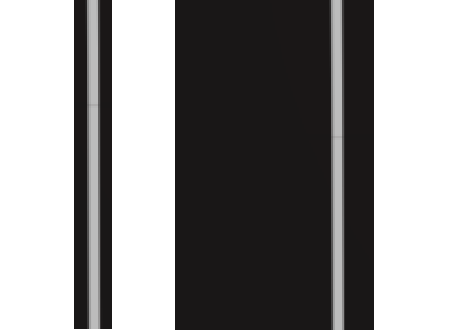
\includegraphics[width=.5\textwidth]{img/roi_breite}
	\caption[unterschiedlich Breite RoI]{unterschiedlich Breite RoI}
	%\captionsource{So könnte man z.b. die Bildquelle angeben}
	\label{fig:vector_kurve}
\end{figure}

\subsection{Unterabschnitt 4}
\Blindtext\Blindtext

\section{Hauptteil 2}

\subsection{Unterabschnitt}
\blindtext
\begin{quote}
	„Beispielzitat 1“ \cite{knuth:1984} \cite{IEEEexample:texfaq}
\end{quote}

\begin{formal}
	Falls Sie doch mal ein Vollzitat verwenden sollten um zum Beispiel eine Definition nach einem 		    bestimmten Werk anzugeben können Sie das so machen.
	\begin{flushright}
		\textit{--- Fachbuch XY \cite{IEEEexample:texfaq}}
	\end{flushright}
\end{formal}

\begin{table}[H]
	\centering
	\caption{Beispieltabelle}
	\begin{tabular}{c | c}
		\hline 
		\large{Überschrift1} & \large{Überschrift2} \\
		\hline \\
		Inhalt1 & Inhalt2\\
		Inhalt3 & Inhalt4\\
	\end{tabular}

\end{table}
\subsection{Unterabschnitt}
\blindtext
\subsubsection{Unterunterabschnitt}
\blindtext
\subsubsection{Unterunterabschnitt}
\blindtext
\paragraph{Paragraph}
\blindtext
\paragraph{Paragraph}
\blindtext
\subparagraph{Subparagraph}
\blindtext